\documentclass[10pt,a4paper]{article}
\usepackage[margin=0.6in]{geometry}
\usepackage{amsmath,amssymb,amsthm}
\usepackage{booktabs}
\usepackage{multirow}
\usepackage{xcolor}
\usepackage{tcolorbox}
\tcbuselibrary{breakable}
\usepackage[colorlinks=true,linkcolor=blue]{hyperref}
\usepackage{titlesec}
\usepackage{enumitem}
\usepackage{tikz}
\usepackage{circuitikz}
\usetikzlibrary{shapes,arrows,positioning,calc}

% Color scheme
\definecolor{headcolor}{RGB}{0,102,204}
\definecolor{keycolor}{RGB}{220,20,60}
\definecolor{solutioncolor}{RGB}{34,139,34}
\definecolor{mnemoniccolor}{RGB}{148,0,211}

% Custom environments
\newtcolorbox{solutionbox}{
 breakable,
 colback=solutioncolor!5!white,
 colframe=solutioncolor!75!black,
 fonttitle=\bfseries,
 title=Solution
}

\newtcolorbox{keyformula}{
 colback=keycolor!5!white,
 colframe=keycolor!75!black,
 fonttitle=\bfseries,
 title=Key Formula
}

\newtcolorbox{mnemonicbox}{
 colback=mnemoniccolor!5!white,
 colframe=mnemoniccolor!75!black,
 fonttitle=\bfseries,
 title=Mnemonic
}

% Spacing
\setlength{\parskip}{3pt}
\setlist[itemize]{nosep}
\setlist[enumerate]{nosep}

% Title formatting
\titleformat{\section}{\Large\bfseries\color{headcolor}}{\thesection}{1em}{}
\titleformat{\subsection}{\large\bfseries\color{headcolor}}{\thesubsection}{1em}{}

\begin{document}

\begin{center}
{\Huge\bfseries\color{headcolor} Modern Physics Solutions}\\[5pt]
{\LARGE DI01000061 -- Winter 2024}\\[3pt]
{\large Semester 1 Study Material}\\[3pt]
{\normalsize\textit{Detailed Solutions and Explanations}}
\end{center}

\vspace{10pt}

%----------------------------------------
\section*{Question 1 -- Fill in the blanks/MCQs [14 marks]}

\begin{solutionbox}
\textbf{Answer Table:}

\begin{center}
\begin{tabular}{|c|c|c|c|}
\hline
\textbf{Question} & \textbf{Answer} & \textbf{Question} & \textbf{Answer} \\
\hline
(1) & (a) Si & (8) & (b) 0.5 Hz \\
(2) & (a) 1.50 & (9) & (a) 300000 km/s \\
(3) & (b) greater than & (10) & (b) solid \\
(4) & (c) 4 & (11) & (a) crest and trough \\
(5) & (d) Total internal reflection & (12) & (b) monochromatic \\
(6) & (d) frequency & (13) & (a) Single mode \\
(7) & (a) Coulomb & (14) & (b) 45° \\
\hline
\end{tabular}
\end{center}
\end{solutionbox}

\begin{mnemonicbox}
``Silicon Glass Bridge Optic Frequency Coulomb Hz Solid Crest Mono Single 45''
\end{mnemonicbox}

%----------------------------------------
\section*{Question 2(A) -- Attempt any two [6 marks]}

\subsection*{Question 2(A)(1) [3 marks]}
\textbf{Differentiate between accuracy and precision.}

\begin{solutionbox}
\begin{center}
\begin{tabular}{|l|p{5.5cm}|p{5.5cm}|}
\hline
\textbf{Parameter} & \textbf{Accuracy} & \textbf{Precision} \\
\hline
Definition & Closeness to true value & Consistency of repeated measurements \\
\hline
Focus & Correctness & Reproducibility \\
\hline
Error Type & Systematic error & Random error \\
\hline
Example & Hitting bullseye & Hitting same spot repeatedly \\
\hline
\end{tabular}
\end{center}

\textbf{Key Points:}
\begin{itemize}
\item \textbf{Accuracy}: How close measurement is to actual value
\item \textbf{Precision}: How close repeated measurements are to each other
\end{itemize}
\end{solutionbox}

\begin{mnemonicbox}
``Accurate Aims Actual, Precise Repeats Reliably''
\end{mnemonicbox}

\subsection*{Question 2(A)(2) [3 marks]}
\textbf{Determine the diameter of a sphere measured by micrometer screw, main scale reading is 5 mm and 50th division of circular scale is coinciding with base line. The least count of this instrument is 0.01 mm.}

\begin{solutionbox}
\textbf{Given:}
\begin{align*}
\text{Main Scale Reading (MSR)} &= 5\text{ mm}\\
\text{Circular Scale Reading (CSR)} &= 50\text{ divisions}\\
\text{Least Count (LC)} &= 0.01\text{ mm}
\end{align*}

\textbf{Formula:}
\[\text{Total Reading} = \text{MSR} + (\text{CSR} \times \text{LC})\]

\textbf{Calculation:}
\begin{align*}
\text{Total Reading} &= 5 + (50 \times 0.01)\\
&= 5 + 0.5\\
&= 5.5\text{ mm}
\end{align*}

\textbf{Answer: Diameter of sphere = 5.5 mm}
\end{solutionbox}

\begin{mnemonicbox}
``Main Scale Reading + Circular $\times$ Least Count''
\end{mnemonicbox}

\subsection*{Question 2(A)(3) [3 marks]}
\textbf{Calculate the amount of electric charge stored on either plate of a capacitor of capacitance 4 µF when connected across 12 volt battery.}

\begin{solutionbox}
\textbf{Given:}
\begin{align*}
\text{Capacitance } (C) &= 4\text{ µF} = 4 \times 10^{-6}\text{ F}\\
\text{Voltage } (V) &= 12\text{ V}
\end{align*}

\begin{keyformula}
\[Q = CV\]
\end{keyformula}

\textbf{Calculation:}
\begin{align*}
Q &= 4 \times 10^{-6} \times 12\\
&= 48 \times 10^{-6}\text{ C}\\
&= 48\text{ µC}
\end{align*}

\textbf{Answer: Electric charge stored = 48 µC}
\end{solutionbox}

\begin{mnemonicbox}
``Charge equals Capacitance times Voltage''
\end{mnemonicbox}

%----------------------------------------
\section*{Question 2(B) -- Attempt any two [8 marks]}

\subsection*{Question 2(B)(1) [4 marks]}
\textbf{Draw a sketch of micrometer screw gauge with proper nomenclature.}

\begin{solutionbox}
\textbf{Micrometer Screw Gauge Diagram:}

\begin{center}
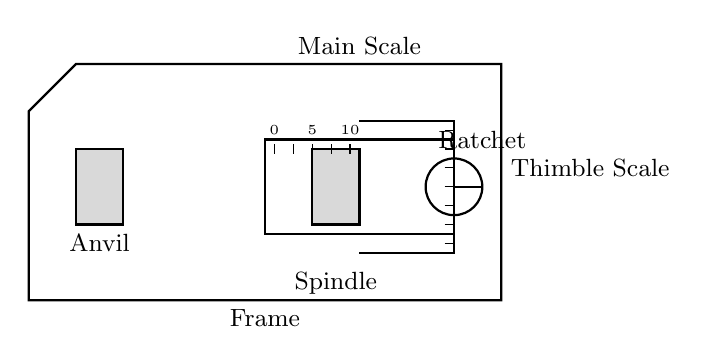
\begin{tikzpicture}[scale=1.2]
% Frame
\draw[thick] (0,0) -- (0,2) -- (0.5,2.5) -- (5,2.5) -- (5,0) -- cycle;
% Anvil (fixed)
\draw[fill=gray!30,thick] (0.5,0.8) rectangle (1,1.6);
% Spindle (movable)
\draw[fill=gray!30,thick] (3,0.8) rectangle (3.5,1.6);
% Main sleeve/barrel
\draw[thick] (2.5,0.7) rectangle (4.5,1.7);
% Thimble
\draw[thick] (3.5,0.5) -- (4.5,0.5) -- (4.5,1.9) -- (3.5,1.9);
% Ratchet
\draw[thick] (4.5,1.2) circle (0.3);
\draw[thick] (4.5,1.2) -- (4.8,1.2);
\draw[thick] (4.5,1.2) -- (4.5,1.5);
\draw[thick] (4.5,1.2) -- (4.5,0.9);

% Labels
\node[below] at (0.75,0.8) {\small Anvil};
\node[below] at (3.25,0.4) {\small Spindle};
\node[above] at (3.5,2.5) {\small Main Scale};
\node[right] at (5,1.4) {\small Thimble Scale};
\node[above] at (4.8,1.5) {\small Ratchet};
\node[below] at (2.5,0) {\small Frame};

% Main scale markings
\foreach \x in {2.6,2.8,3.0,3.2,3.4}
    \draw (\x,1.65) -- (\x,1.55);
\node[above,font=\tiny] at (2.6,1.65) {0};
\node[above,font=\tiny] at (3.0,1.65) {5};
\node[above,font=\tiny] at (3.4,1.65) {10};

% Thimble scale markings
\foreach \y in {0.6,0.8,1.0,1.2,1.4,1.6,1.8}
    \draw (4.4,\y) -- (4.5,\y);
\end{tikzpicture}
\end{center}

\textbf{Main Components:}
\begin{itemize}
\item \textbf{Frame}: U-shaped structure providing support
\item \textbf{Anvil}: Fixed jaw for placing object
\item \textbf{Spindle}: Movable screw mechanism
\item \textbf{Thimble Scale}: Circular scale with 50 divisions
\item \textbf{Main Scale}: Linear scale in mm
\item \textbf{Ratchet}: For consistent pressure application
\end{itemize}
\end{solutionbox}

\begin{mnemonicbox}
``Frame Anvil Spindle Thimble Main Ratchet''
\end{mnemonicbox}

\subsection*{Question 2(B)(2) [4 marks]}
\textbf{Explain the zero, positive and negative errors for vernier calipers with proper diagram and list necessary steps to remove these types of errors.}

\begin{solutionbox}
\textbf{Types of Errors:}

\begin{center}
\begin{tabular}{|l|p{5cm}|p{4cm}|}
\hline
\textbf{Error Type} & \textbf{Condition} & \textbf{Reading} \\
\hline
Zero Error & Zero line of vernier doesn't coincide with main scale zero & Non-zero when jaws closed \\
\hline
Positive Error & Vernier zero is right of main scale zero & Add correction \\
\hline
Negative Error & Vernier zero is left of main scale zero & Subtract correction \\
\hline
\end{tabular}
\end{center}

\vspace{5pt}
\textbf{Diagrams:}

\begin{center}
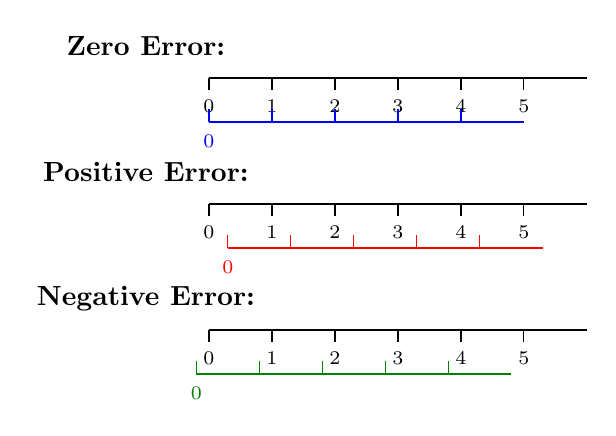
\begin{tikzpicture}[scale=0.8]
% Zero Error
\node at (-1,2) {\textbf{Zero Error:}};
\draw[thick] (0,1.5) -- (6,1.5);
\foreach \x in {0,1,2,3,4,5}
    \draw (\x,1.5) -- (\x,1.3) node[below,font=\scriptsize] {\x};
\draw[thick,blue] (0,0.8) -- (5,0.8);
\foreach \x in {0,1,2,3,4}
    \draw[blue] (\x,0.8) -- (\x,1.0);
\node[blue] at (0,0.5) {\scriptsize 0};

% Positive Error
\node at (-1,0) {\textbf{Positive Error:}};
\draw[thick] (0,-0.5) -- (6,-0.5);
\foreach \x in {0,1,2,3,4,5}
    \draw (\x,-0.5) -- (\x,-0.7) node[below,font=\scriptsize] {\x};
\draw[thick,red] (0.3,-1.2) -- (5.3,-1.2);
\foreach \x in {0.3,1.3,2.3,3.3,4.3}
    \draw[red] (\x,-1.2) -- (\x,-1.0);
\node[red] at (0.3,-1.5) {\scriptsize 0};

% Negative Error  
\node at (-1,-2) {\textbf{Negative Error:}};
\draw[thick] (0,-2.5) -- (6,-2.5);
\foreach \x in {0,1,2,3,4,5}
    \draw (\x,-2.5) -- (\x,-2.7) node[below,font=\scriptsize] {\x};
\draw[thick,green!50!black] (-0.2,-3.2) -- (4.8,-3.2);
\foreach \x in {-0.2,0.8,1.8,2.8,3.8}
    \draw[green!50!black] (\x,-3.2) -- (\x,-3.0);
\node[green!50!black] at (-0.2,-3.5) {\scriptsize 0};
\end{tikzpicture}
\end{center}

\textbf{Steps to Remove Errors:}
\begin{enumerate}
\item \textbf{Check zero error} before measurement
\item \textbf{Apply correction} to final reading
\item \textbf{Clean jaws} regularly to prevent debris
\item \textbf{Handle carefully} to avoid mechanical damage
\end{enumerate}
\end{solutionbox}

\begin{mnemonicbox}
``Check Clean Correct Carefully''
\end{mnemonicbox}

\subsection*{Question 2(B)(3) [4 marks]}
\textbf{In an experiment of finding the periodic time of a simple pendulum, the observations are 1.96 s, 1.98 s, 2.00 s, 2.02 s, 2.04 s. Calculate absolute error, mean absolute error, relative error and percentage error.}

\begin{solutionbox}
\textbf{Observations:} 1.96, 1.98, 2.00, 2.02, 2.04 s

\textbf{Mean value:}
\[\bar{x} = \frac{1.96 + 1.98 + 2.00 + 2.02 + 2.04}{5} = \frac{10.00}{5} = 2.00\text{ s}\]

\textbf{Absolute errors:} $|x_i - \bar{x}|$
\begin{center}
\begin{tabular}{|c|c|c|}
\hline
\textbf{Observation} & \textbf{Value (s)} & \textbf{Absolute Error (s)} \\
\hline
1 & 1.96 & $|1.96 - 2.00| = 0.04$ \\
2 & 1.98 & $|1.98 - 2.00| = 0.02$ \\
3 & 2.00 & $|2.00 - 2.00| = 0.00$ \\
4 & 2.02 & $|2.02 - 2.00| = 0.02$ \\
5 & 2.04 & $|2.04 - 2.00| = 0.04$ \\
\hline
\end{tabular}
\end{center}

\textbf{Mean absolute error:}
\[\Delta x_{\text{mean}} = \frac{0.04 + 0.02 + 0.00 + 0.02 + 0.04}{5} = \frac{0.12}{5} = 0.024\text{ s}\]

\textbf{Relative error:}
\[\text{Relative error} = \frac{\Delta x_{\text{mean}}}{\bar{x}} = \frac{0.024}{2.00} = 0.012\]

\textbf{Percentage error:}
\[\text{Percentage error} = \text{Relative error} \times 100 = 0.012 \times 100 = 1.2\%\]

\textbf{Results:}
\begin{itemize}
\item Mean absolute error = 0.024 s
\item Relative error = 0.012
\item Percentage error = 1.2\%
\end{itemize}
\end{solutionbox}

\begin{mnemonicbox}
``Mean Absolute Relative Percentage''
\end{mnemonicbox}

%----------------------------------------
\section*{Question 3(A) -- Attempt any two [6 marks]}

\subsection*{Question 3(A)(1) [3 marks]}
\textbf{Define: Electric flux, Electric field, Potential Difference}

\begin{solutionbox}
\begin{center}
\begin{tabular}{|l|p{4.5cm}|c|c|}
\hline
\textbf{Term} & \textbf{Definition} & \textbf{Unit} & \textbf{Formula} \\
\hline
Electric Flux & Number of electric field lines passing through a surface & Nm²/C & $\Phi = E \cdot A$ \\
\hline
Electric Field & Force per unit positive charge & N/C & $E = F/q$ \\
\hline
Potential Difference & Work done per unit charge between two points & Volt & $V = W/q$ \\
\hline
\end{tabular}
\end{center}

\textbf{Key Points:}
\begin{itemize}
\item \textbf{Electric flux}: Measure of field lines penetrating surface
\item \textbf{Electric field}: Region where electric force acts on charges
\item \textbf{Potential difference}: Energy difference per unit charge
\end{itemize}
\end{solutionbox}

\begin{mnemonicbox}
``Flux Field Force, Work Watts Volts''
\end{mnemonicbox}

\subsection*{Question 3(A)(2) [3 marks]}
\textbf{Derive the formula for equivalent capacitance when three different capacitors are connected in series with necessary circuit diagram.}

\begin{solutionbox}
\textbf{Circuit Diagram:}

\begin{center}
\begin{circuitikz}
\draw (0,2) to[C=$C_1$] (2,2)
           to[C=$C_2$] (4,2)
           to[C=$C_3$] (6,2);
\draw (0,2) to[short,o-] (0,2) node[left] {$+$};
\draw (6,2) to[short,-o] (6,2) node[right] {$-$};
\draw (0,0) to[short,o-] (6,0) to[short,-o] (6,0);
\draw (0,0) -- (0,2);
\draw (6,0) -- (6,2);
\node at (3,-0.5) {$V$};
\end{circuitikz}
\end{center}

\textbf{Derivation:}
\begin{itemize}
\item \textbf{Same charge} $Q$ flows through each capacitor
\item \textbf{Voltage divides}: $V = V_1 + V_2 + V_3$
\item \textbf{For each capacitor}: $V_1 = Q/C_1$, $V_2 = Q/C_2$, $V_3 = Q/C_3$
\item \textbf{Total voltage}: 
\[V = \frac{Q}{C_1} + \frac{Q}{C_2} + \frac{Q}{C_3} = Q\left(\frac{1}{C_1} + \frac{1}{C_2} + \frac{1}{C_3}\right)\]
\item \textbf{For equivalent}: $V = Q/C_s$
\item \textbf{Therefore}: 
\end{itemize}

\begin{keyformula}
\[\frac{1}{C_s} = \frac{1}{C_1} + \frac{1}{C_2} + \frac{1}{C_3}\]
\end{keyformula}
\end{solutionbox}

\begin{mnemonicbox}
``Series Sums reciprocals, Same charge Splits voltage''
\end{mnemonicbox}

\subsection*{Question 3(A)(3) [3 marks]}
\textbf{Define: Infrasonic sound, Audible Sound, Ultrasonic sound}

\begin{solutionbox}
\begin{center}
\begin{tabular}{|l|c|p{3.5cm}|p{3cm}|}
\hline
\textbf{Sound Type} & \textbf{Frequency Range} & \textbf{Characteristics} & \textbf{Applications} \\
\hline
Infrasonic & Below 20 Hz & Inaudible to humans & Earthquake detection \\
\hline
Audible & 20 Hz to 20 kHz & Audible to humans & Communication, music \\
\hline
Ultrasonic & Above 20 kHz & Inaudible to humans & Medical imaging, SONAR \\
\hline
\end{tabular}
\end{center}

\textbf{Key Points:}
\begin{itemize}
\item \textbf{Infrasonic}: Low frequency sounds below human hearing
\item \textbf{Audible}: Normal hearing range for humans
\item \textbf{Ultrasonic}: High frequency sounds above human hearing
\end{itemize}
\end{solutionbox}

\begin{mnemonicbox}
``Infra-Below, Audible-Between, Ultra-Above''
\end{mnemonicbox}

%----------------------------------------
\section*{Question 3(B) -- Attempt any two [8 marks]}

\subsection*{Question 3(B)(1) [4 marks]}
\textbf{Prove $C = \epsilon_0 A/d$ for parallel plate capacitor.}

\begin{solutionbox}
\textbf{Diagram:}

\begin{center}
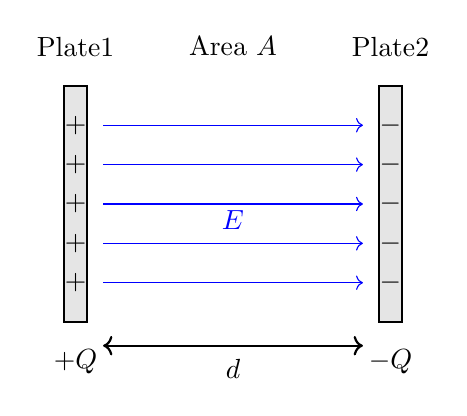
\begin{tikzpicture}
% Plates
\draw[thick,fill=gray!20] (0,0) rectangle (0.3,3);
\draw[thick,fill=gray!20] (4,0) rectangle (4.3,3);
% Charges
\node at (0.15,2.5) {$+$};
\node at (0.15,2) {$+$};
\node at (0.15,1.5) {$+$};
\node at (0.15,1) {$+$};
\node at (0.15,0.5) {$+$};
\node at (4.15,2.5) {$-$};
\node at (4.15,2) {$-$};
\node at (4.15,1.5) {$-$};
\node at (4.15,1) {$-$};
\node at (4.15,0.5) {$-$};
% Labels
\node at (0.15,3.5) {Plate1};
\node at (4.15,3.5) {Plate2};
\node at (0.15,-0.5) {$+Q$};
\node at (4.15,-0.5) {$-Q$};
\node at (2.15,3.5) {Area $A$};
% Distance
\draw[<->,thick] (0.5,-0.3) -- (3.8,-0.3);
\node at (2.15,-0.6) {$d$};
% Field lines
\foreach \y in {0.5,1,1.5,2,2.5}
    \draw[->,blue] (0.5,\y) -- (3.8,\y);
\node[blue] at (2.15,1.3) {$E$};
\end{tikzpicture}
\end{center}

\textbf{Derivation:}
\begin{itemize}
\item \textbf{Electric field} between plates: 
\[E = \frac{\sigma}{\epsilon_0} = \frac{Q}{\epsilon_0 A}\]
where $\sigma = Q/A$ is surface charge density

\item \textbf{Potential difference}: 
\[V = E \times d = \frac{Qd}{\epsilon_0 A}\]

\item \textbf{Capacitance definition}: $C = Q/V$

\item \textbf{Substituting}: 
\[C = \frac{Q}{Qd/(\epsilon_0 A)} = \frac{\epsilon_0 A}{d}\]
\end{itemize}

\begin{keyformula}
\[C = \frac{\epsilon_0 A}{d}\]
Where: $\epsilon_0$ = Permittivity of free space, $A$ = Area of plates, $d$ = Distance between plates
\end{keyformula}
\end{solutionbox}

\begin{mnemonicbox}
``Capacitance equals epsilon-zero Area over distance''
\end{mnemonicbox}

\subsection*{Question 3(B)(2) [4 marks]}
\textbf{List the characteristics of electric field lines.}

\begin{solutionbox}
\textbf{Key Characteristics:}
\begin{enumerate}
\item \textbf{Direction}: From positive to negative charge
\item \textbf{Density}: Indicates field strength
\item \textbf{Continuous}: Never break in free space
\item \textbf{Non-intersecting}: No two lines cross
\item \textbf{Perpendicular}: To conductor surface
\item \textbf{Closed loops}: Only around changing magnetic fields
\item \textbf{Tangent}: Gives field direction at any point
\item \textbf{Uniform spacing}: In uniform field regions
\end{enumerate}

\textbf{Properties:}
\begin{itemize}
\item Start from \textbf{positive charges}
\item End at \textbf{negative charges}
\item \textbf{Higher density} means stronger field
\item \textbf{Never intersect} each other
\end{itemize}
\end{solutionbox}

\begin{mnemonicbox}
``Positive to Negative, Dense means Strong, Never cross, Always perpendicular''
\end{mnemonicbox}

\subsection*{Question 3(B)(3) [4 marks]}
\textbf{Describe working and construction of magnetostriction method used for production of ultrasonic waves.}

\begin{solutionbox}
\textbf{Construction Block Diagram:}

\begin{center}
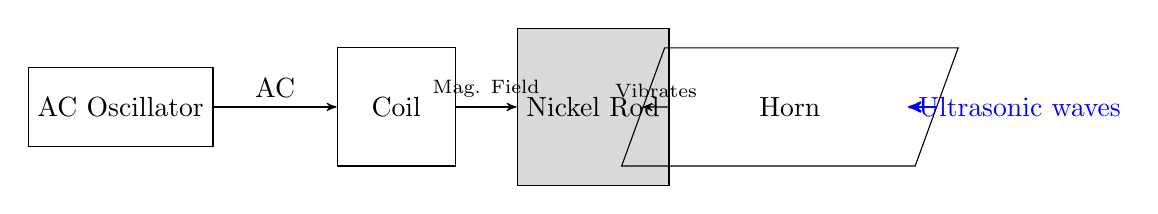
\begin{tikzpicture}[node distance=2cm,auto,>=stealth']
\node[draw,rectangle,minimum height=1cm,minimum width=2cm] (osc) {AC Oscillator};
\node[draw,rectangle,minimum height=1.5cm,minimum width=1.5cm,right of=osc,node distance=3.5cm] (coil) {Coil};
\node[draw,rectangle,fill=gray!30,minimum height=2cm,minimum width=0.8cm,right of=coil,node distance=2.5cm] (rod) {Nickel Rod};
\node[draw,trapezium,trapezium left angle=70,trapezium right angle=110,minimum height=1.5cm,right of=rod,node distance=2.5cm] (horn) {Horn};

\draw[->] (osc) -- (coil) node[midway,above] {AC};
\draw[->] (coil) -- (rod) node[midway,above,font=\scriptsize] {Mag. Field};
\draw[->] (rod) -- (horn) node[midway,above,font=\scriptsize] {Vibrates};
\draw[->,thick,blue] (horn) -- ++(1.5,0) node[right] {Ultrasonic waves};
\end{tikzpicture}
\end{center}

\textbf{Components:}
\begin{itemize}
\item \textbf{Nickel rod}: Magnetostrictive material
\item \textbf{Coil}: Electromagnet around rod
\item \textbf{AC oscillator}: High frequency current source
\item \textbf{Horn}: Sound amplifier and transmitter
\end{itemize}

\textbf{Working Principle:}
\begin{enumerate}
\item \textbf{AC current} flows through coil
\item \textbf{Magnetic field} changes rapidly
\item \textbf{Nickel rod} expands and contracts (magnetostriction effect)
\item \textbf{Mechanical vibrations} produced at high frequency
\item \textbf{Ultrasonic waves} generated and amplified by horn
\end{enumerate}

\textbf{Applications}: Medical imaging, cleaning, welding, material testing
\end{solutionbox}

\begin{mnemonicbox}
``AC Coil Makes Nickel vibrate, Creates Ultrasonic''
\end{mnemonicbox}

%----------------------------------------
\section*{Question 4(A) -- Attempt any two [6 marks]}

\subsection*{Question 4(A)(1) [3 marks]}
\textbf{A radio station broadcasts its radio signals at $9.26 \times 10^7$ Hz. Find the wavelength if the waves travel at a speed of $3.00 \times 10^8$ m/s.}

\begin{solutionbox}
\textbf{Given:}
\begin{align*}
\text{Frequency } (f) &= 9.26 \times 10^7\text{ Hz}\\
\text{Speed } (c) &= 3.00 \times 10^8\text{ m/s}
\end{align*}

\begin{keyformula}
\[c = f\lambda \quad \Rightarrow \quad \lambda = \frac{c}{f}\]
\end{keyformula}

\textbf{Calculation:}
\begin{align*}
\lambda &= \frac{3.00 \times 10^8}{9.26 \times 10^7}\\
&= \frac{3.00}{9.26} \times 10^{8-7}\\
&= 0.324 \times 10^1\\
&= 3.24\text{ m}
\end{align*}

\textbf{Answer: Wavelength = 3.24 m}
\end{solutionbox}

\begin{mnemonicbox}
``Speed equals frequency times wavelength''
\end{mnemonicbox}

\subsection*{Question 4(A)(2) [3 marks]}
\textbf{State the Snell's law and explain refractive index of media.}

\begin{solutionbox}
\begin{keyformula}
\textbf{Snell's Law:}
\[n_1 \sin\theta_1 = n_2 \sin\theta_2\]
\end{keyformula}

Where: $n_1, n_2$ = Refractive indices of media 1 and 2, $\theta_1, \theta_2$ = Angles of incidence and refraction

\vspace{5pt}
\textbf{Refractive Index:}

\begin{center}
\begin{tabular}{|l|p{4.5cm}|c|}
\hline
\textbf{Type} & \textbf{Definition} & \textbf{Formula} \\
\hline
Absolute & Speed of light in vacuum to medium & $n = c/v$ \\
\hline
Relative & Ratio of speeds in two media & $n_{21} = v_1/v_2$ \\
\hline
\end{tabular}
\end{center}

\textbf{Key Points:}
\begin{itemize}
\item \textbf{Higher refractive index}: Denser medium, slower light
\item \textbf{Lower refractive index}: Rarer medium, faster light
\end{itemize}
\end{solutionbox}

\begin{mnemonicbox}
``Snell Says Sine ratio constant, Dense slows Down light''
\end{mnemonicbox}

\subsection*{Question 4(A)(3) [3 marks]}
\textbf{Compare: Ordinary light and LASER}

\begin{solutionbox}
\begin{center}
\begin{tabular}{|l|p{4.5cm}|p{4.5cm}|}
\hline
\textbf{Property} & \textbf{Ordinary Light} & \textbf{LASER} \\
\hline
Coherence & Incoherent & Coherent \\
\hline
Color & Polychromatic & Monochromatic \\
\hline
Direction & Divergent & Parallel beam \\
\hline
Intensity & Low & Very high \\
\hline
Phase & Random & Fixed phase relationship \\
\hline
Wavelength & Multiple wavelengths & Single wavelength \\
\hline
\end{tabular}
\end{center}

\textbf{Key Differences:}
\begin{itemize}
\item \textbf{LASER}: Coherent, monochromatic, parallel, intense
\item \textbf{Ordinary}: Incoherent, polychromatic, divergent, less intense
\end{itemize}
\end{solutionbox}

\begin{mnemonicbox}
``LASER: Coherent Monochromatic Parallel Intense''
\end{mnemonicbox}

%----------------------------------------
\section*{Question 4(B) -- Attempt any two [8 marks]}

\subsection*{Question 4(B)(1) [4 marks]}
\textbf{Demonstrate the structure of an optical fiber with necessary diagram.}

\begin{solutionbox}
\textbf{Optical Fiber Structure:}

\begin{center}
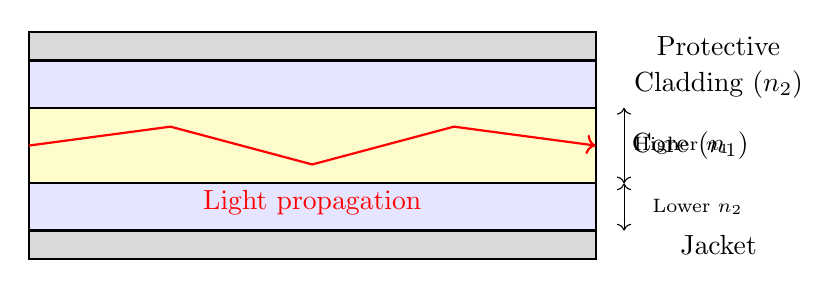
\begin{tikzpicture}[scale=1.2]
% Core
\draw[thick,fill=yellow!20] (0,1) rectangle (6,1.8);
\node at (7,1.4) {Core ($n_1$)};
% Cladding - upper
\draw[thick,fill=blue!10] (0,1.8) rectangle (6,2.3);
\node at (7.3,2.05) {Cladding ($n_2$)};
% Cladding - lower
\draw[thick,fill=blue!10] (0,0.5) rectangle (6,1);
% Jacket - upper
\draw[thick,fill=gray!30] (0,2.3) rectangle (6,2.6);
\node at (7.3,2.45) {Protective};
% Jacket - lower
\draw[thick,fill=gray!30] (0,0.2) rectangle (6,0.5);
\node at (7.3,0.35) {Jacket};
% Light ray
\draw[->,red,thick] (0,1.4) -- (1.5,1.6) -- (3,1.2) -- (4.5,1.6) -- (6,1.4);
\node[red] at (3,0.8) {Light propagation};
% Labels
\draw[<->] (6.3,1) -- (6.3,1.8);
\node[right] at (6.3,1.4) {\scriptsize Higher $n_1$};
\draw[<->] (6.3,0.5) -- (6.3,1.0);
\node[right] at (6.5,0.75) {\scriptsize Lower $n_2$};
\end{tikzpicture}
\end{center}

\textbf{Components:}

\begin{center}
\begin{tabular}{|l|l|p{4cm}|c|}
\hline
\textbf{Component} & \textbf{Material} & \textbf{Function} & \textbf{Ref. Index} \\
\hline
Core & Glass/Plastic & Light transmission & Higher ($n_1$) \\
\hline
Cladding & Glass & Total internal reflection & Lower ($n_2$) \\
\hline
Jacket & Plastic & Protection & -- \\
\hline
\end{tabular}
\end{center}

\textbf{Working Principle:}
\begin{itemize}
\item Light enters \textbf{core} at acceptance angle
\item \textbf{Total internal reflection} at core-cladding boundary
\item Light travels in \textbf{zigzag path} through core
\item \textbf{$n_1 > n_2$} ensures light confinement
\end{itemize}
\end{solutionbox}

\begin{mnemonicbox}
``Core Cladding Jacket, Higher Lower Protection''
\end{mnemonicbox}

\subsection*{Question 4(B)(2) [4 marks]}
\textbf{List applications of LASER in engineering and medical field.}

\begin{solutionbox}
\textbf{Engineering Applications:}
\begin{enumerate}
\item \textbf{Cutting and welding}: Precision metal cutting
\item \textbf{3D printing}: Laser sintering
\item \textbf{Measurement}: Distance and surveying
\item \textbf{Communication}: Optical fiber systems
\item \textbf{Material processing}: Surface hardening
\item \textbf{Barcode scanning}: Retail and inventory
\end{enumerate}

\textbf{Medical Applications:}
\begin{enumerate}
\item \textbf{Surgery}: Precise tissue cutting
\item \textbf{Eye treatment}: Corrective surgery
\item \textbf{Cancer treatment}: Tumor destruction
\item \textbf{Diagnostics}: Spectroscopy
\item \textbf{Dentistry}: Cavity treatment
\item \textbf{Skin treatment}: Cosmetic procedures
\end{enumerate}

\textbf{Advantages}: Precision, non-contact, sterile, minimal damage
\end{solutionbox}

\begin{mnemonicbox}
``Engineering: Cut Weld Measure Communicate, Medical: Surgery Eye Cancer Diagnose''
\end{mnemonicbox}

\subsection*{Question 4(B)(3) [4 marks]}
\textbf{Explain P-type and N-type semiconductors.}

\begin{solutionbox}
\textbf{N-type Semiconductor:}

\begin{center}
\begin{tabular}{|l|p{8cm}|}
\hline
\textbf{Property} & \textbf{N-type} \\
\hline
Dopant & Phosphorus, Arsenic (5 valence electrons) \\
\hline
Majority carriers & Electrons \\
\hline
Minority carriers & Holes \\
\hline
Charge & Negative \\
\hline
\end{tabular}
\end{center}

\textbf{P-type Semiconductor:}

\begin{center}
\begin{tabular}{|l|p{8cm}|}
\hline
\textbf{Property} & \textbf{P-type} \\
\hline
Dopant & Boron, Aluminum (3 valence electrons) \\
\hline
Majority carriers & Holes \\
\hline
Minority carriers & Electrons \\
\hline
Charge & Positive \\
\hline
\end{tabular}
\end{center}

\textbf{Formation Process:}
\begin{itemize}
\item \textbf{N-type}: Pentavalent atoms donate electrons
\item \textbf{P-type}: Trivalent atoms accept electrons, create holes
\item \textbf{Doping}: Controlled addition of impurities
\item \textbf{Conductivity}: Increases due to free carriers
\end{itemize}
\end{solutionbox}

\begin{mnemonicbox}
``N-type Negative electrons, P-type Positive holes''
\end{mnemonicbox}

%----------------------------------------
\section*{Question 5(A) -- Attempt any two [6 marks]}

\subsection*{Question 5(A)(1) [3 marks]}
\textbf{Classify conductors, semiconductors and insulators based on energy band gap.}

\begin{solutionbox}
\begin{center}
\begin{tabular}{|l|c|p{3.5cm}|p{3cm}|}
\hline
\textbf{Material} & \textbf{Energy Band Gap} & \textbf{Characteristics} & \textbf{Examples} \\
\hline
Conductor & No gap (0 eV) & Valence and conduction bands overlap & Copper, Silver \\
\hline
Semiconductor & Small gap (1-3 eV) & Moderate band gap & Silicon, Germanium \\
\hline
Insulator & Large gap ($>$3 eV) & Wide band gap & Glass, Rubber \\
\hline
\end{tabular}
\end{center}

\textbf{Energy Band Diagram:}

\begin{center}
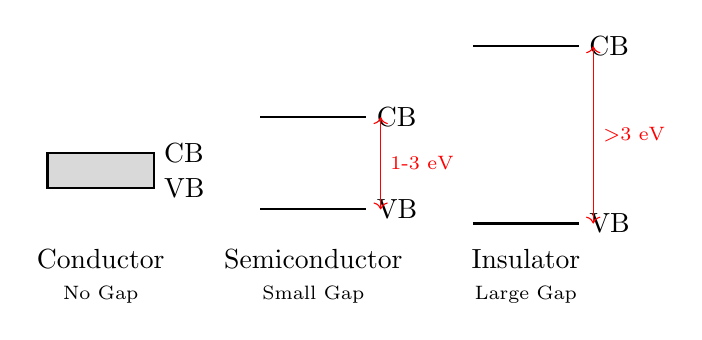
\begin{tikzpicture}[scale=0.9]
% Conductor
\draw[thick] (0,2) -- (1.5,2) node[right] {CB};
\draw[thick,fill=gray!30] (0,1.5) rectangle (1.5,2);
\draw[thick,fill=gray!30] (0,1.5) -- (1.5,1.5) node[right] {VB};
\node at (0.75,0.5) {Conductor};
\node at (0.75,0) {\scriptsize No Gap};

% Semiconductor
\draw[thick] (3,2.5) -- (4.5,2.5) node[right] {CB};
\draw[thick] (3,1.2) -- (4.5,1.2) node[right] {VB};
\draw[<->,red] (4.7,1.2) -- (4.7,2.5) node[midway,right] {\scriptsize 1-3 eV};
\node at (3.75,0.5) {Semiconductor};
\node at (3.75,0) {\scriptsize Small Gap};

% Insulator
\draw[thick] (6,3.5) -- (7.5,3.5) node[right] {CB};
\draw[thick] (6,1.0) -- (7.5,1.0) node[right] {VB};
\draw[<->,red] (7.7,1.0) -- (7.7,3.5) node[midway,right] {\scriptsize $>$3 eV};
\node at (6.75,0.5) {Insulator};
\node at (6.75,0) {\scriptsize Large Gap};
\end{tikzpicture}
\end{center}

\textbf{Key Points:}
\begin{itemize}
\item \textbf{CB}: Conduction Band, \textbf{VB}: Valence Band
\item \textbf{Gap determines} electrical conductivity
\end{itemize}
\end{solutionbox}

\begin{mnemonicbox}
``No gap Conducts, Small gap Semi, Large gap Insulates''
\end{mnemonicbox}

\subsection*{Question 5(A)(2) [3 marks]}
\textbf{Explain OR and AND logic gates with necessary truth table.}

\begin{solutionbox}
\textbf{OR Gate:}

\begin{minipage}{0.45\textwidth}
\begin{center}
\begin{tabular}{|c|c|c|}
\hline
\textbf{A} & \textbf{B} & \textbf{Y = A + B} \\
\hline
0 & 0 & 0 \\
0 & 1 & 1 \\
1 & 0 & 1 \\
1 & 1 & 1 \\
\hline
\end{tabular}
\end{center}
\end{minipage}
\hfill
\begin{minipage}{0.45\textwidth}
\begin{center}
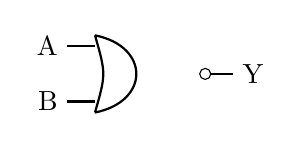
\begin{tikzpicture}[scale=0.7]
\draw[thick] (0,0.5) -- (0.5,0.5);
\draw[thick] (0,1.5) -- (0.5,1.5);
\draw[thick] (0.5,0.3) .. controls (1.5,0.5) and (1.5,1.5) .. (0.5,1.7);
\draw[thick] (0.5,0.3) .. controls (0.7,1) .. (0.5,1.7);
\draw[thick] (2.5,1) -- (3,1);
\node[left] at (0,1.5) {A};
\node[left] at (0,0.5) {B};
\node[right] at (3,1) {Y};
\draw[fill=white] (2.5,1) circle (0.1);
\end{tikzpicture}
\end{center}
\end{minipage}

\vspace{10pt}
\textbf{AND Gate:}

\begin{minipage}{0.45\textwidth}
\begin{center}
\begin{tabular}{|c|c|c|}
\hline
\textbf{A} & \textbf{B} & \textbf{Y = A $\cdot$ B} \\
\hline
0 & 0 & 0 \\
0 & 1 & 0 \\
1 & 0 & 0 \\
1 & 1 & 1 \\
\hline
\end{tabular}
\end{center}
\end{minipage}
\hfill
\begin{minipage}{0.45\textwidth}
\begin{center}
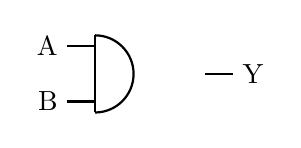
\begin{tikzpicture}[scale=0.7]
\draw[thick] (0,0.5) -- (0.5,0.5) -- (0.5,0.3);
\draw[thick] (0,1.5) -- (0.5,1.5) -- (0.5,1.7);
\draw[thick] (0.5,0.3) -- (0.5,1.7);
\draw[thick] (0.5,0.3) arc (-90:90:0.7);
\draw[thick] (2.5,1) -- (3,1);
\node[left] at (0,1.5) {A};
\node[left] at (0,0.5) {B};
\node[right] at (3,1) {Y};
\end{tikzpicture}
\end{center}
\end{minipage}

\vspace{5pt}
\textbf{Key Points:}
\begin{itemize}
\item \textbf{OR}: Output HIGH when any input is HIGH
\item \textbf{AND}: Output HIGH when all inputs are HIGH
\end{itemize}
\end{solutionbox}

\begin{mnemonicbox}
``OR: Any high makes high, AND: All high makes high''
\end{mnemonicbox}

\subsection*{Question 5(A)(3) [3 marks]}
\textbf{Describe the use of Zener diode as a voltage regulator.}

\begin{solutionbox}
\textbf{Circuit Diagram:}

\begin{center}
\begin{circuitikz}
\draw (0,2) to[short,o-] (1,2) to[R=$R_s$] (3,2) to[short,-o] (4,2);
\draw (3,2) to[short] (3,1.5);
\draw (3,1.5) to[zD,color=red] (3,0);
\draw (3,0) to[short,-o] (4,0) to[short] (0,0) to[short,-o] (0,0);
\node[left] at (0,2) {$V_{in}$};
\node[right] at (4,2) {$V_{out}$};
\node[right] at (4,0) {GND};
\node[red] at (3.8,0.75) {Zener};
\draw[thick] (3.5,2) to[short] (3.5,0);
\node at (4.5,1) {Load};
\end{circuitikz}
\end{center}

\textbf{Working Principle:}
\begin{itemize}
\item \textbf{Forward bias}: Acts like normal diode
\item \textbf{Reverse bias}: Breaks down at Zener voltage
\item \textbf{Voltage regulation}: Maintains constant $V_{out} = V_z$
\item \textbf{Series resistor}: Limits current through Zener
\end{itemize}

\textbf{Characteristics:}
\begin{itemize}
\item \textbf{Zener voltage}: Constant breakdown voltage
\item \textbf{Current range}: Wide operating range
\item \textbf{Temperature stability}: Good voltage stability
\item \textbf{Power rating}: Must not exceed maximum power
\end{itemize}

\textbf{Applications}: Power supplies, voltage references, protection circuits
\end{solutionbox}

\begin{mnemonicbox}
``Zener Zealously maintains Voltage despite Variations''
\end{mnemonicbox}

%----------------------------------------
\section*{Question 5(B) -- Attempt any two [8 marks]}

\subsection*{Question 5(B)(1) [4 marks]}
\textbf{Explain full wave rectifier with necessary circuit and draw input and output waveforms.}

\begin{solutionbox}
\textbf{Center-tap Full Wave Rectifier:}

\begin{center}
\begin{circuitikz}[scale=0.9]
% Transformer
\draw (0,2) to[sinusoidal voltage source] (0,0);
\draw (0,2) -- (0.5,2) -- (0.5,2.5);
\draw (0.5,1.5) -- (0.5,0.5);
\draw (0,0) -- (0.5,0) -- (0.5,0.5);
\draw (1,2.5) -- (1,3) -- (2,3);
\draw (1,1.5) -- (1,1.5);
\draw (1,0.5) -- (1,0) -- (2,0);
% Diodes
\draw (2,3) to[D=$D_1$] (4,3);
\draw (2,0) to[D=$D_2$] (4,0);
% Load
\draw (4,3) to[short] (4.5,3) to[R=$R_L$] (4.5,0) to[short] (4,0);
% Center tap
\draw (1,1.5) to[short] (2,1.5) to[short] (4.5,1.5);
% Output
\draw (4.5,3) to[short,-o] (5,3);
\draw (4.5,0) to[short,-o] (5,0);
\node at (-0.5,1) {AC};
\node at (5.3,3) {$+$};
\node at (5.3,0) {$-$};
\node at (4.5,3.5) {Output};
\end{circuitikz}
\end{center}

\textbf{Working:}
\begin{itemize}
\item \textbf{Positive half cycle}: $D_1$ conducts, $D_2$ off
\item \textbf{Negative half cycle}: $D_2$ conducts, $D_1$ off
\item \textbf{Both halves}: Current flows through load in same direction
\end{itemize}

\textbf{Waveforms:}

\begin{center}
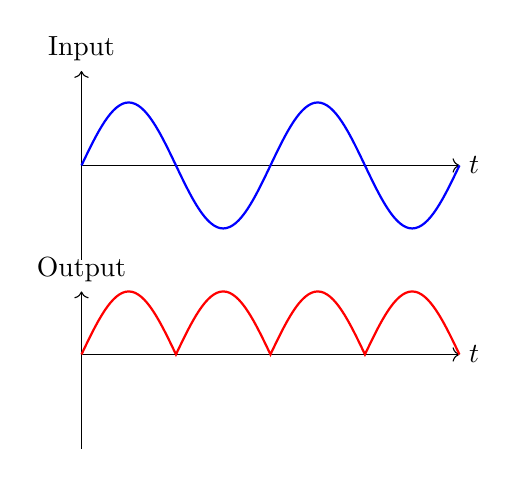
\begin{tikzpicture}[scale=0.8]
% Input waveform
\draw[->] (0,0) -- (6,0) node[right] {$t$};
\draw[->] (0,-1.5) -- (0,1.5) node[above] {Input};
\draw[thick,blue] (0,0) sin (0.75,1) cos (1.5,0) sin (2.25,-1) cos (3,0) sin (3.75,1) cos (4.5,0) sin (5.25,-1) cos (6,0);

% Output waveform
\draw[->] (0,-3) -- (6,-3) node[right] {$t$};
\draw[->] (0,-4.5) -- (0,-2) node[above] {Output};
\draw[thick,red] (0,-3) sin (0.75,-2) cos (1.5,-3) sin (2.25,-2) cos (3,-3) sin (3.75,-2) cos (4.5,-3) sin (5.25,-2) cos (6,-3);
\end{tikzpicture}
\end{center}

\textbf{Advantages}: Better efficiency, lower ripple, better transformer utilization
\end{solutionbox}

\begin{mnemonicbox}
``Full wave uses Full cycle, Better efficiency Better output''
\end{mnemonicbox}

\subsection*{Question 5(B)(2) [4 marks]}
\textbf{Demonstrate forward and reverse characteristics of P-N junction diode.}

\begin{solutionbox}
\textbf{Forward Bias Characteristics:}

\begin{center}
\begin{tabular}{|l|c|l|}
\hline
\textbf{Voltage Range} & \textbf{Current} & \textbf{Behavior} \\
\hline
0 to 0.3V (Si) & Very small & Cut-in voltage \\
\hline
Above 0.7V & Exponential increase & Conducting \\
\hline
\end{tabular}
\end{center}

\textbf{Reverse Bias Characteristics:}

\begin{center}
\begin{tabular}{|l|c|l|}
\hline
\textbf{Voltage Range} & \textbf{Current} & \textbf{Behavior} \\
\hline
0 to breakdown & Reverse saturation & Leakage current \\
\hline
Breakdown voltage & Sharp increase & Avalanche breakdown \\
\hline
\end{tabular}
\end{center}
\end{solutionbox}

\begin{solutionbox}
\textbf{I-V Characteristic Curve:}

\begin{center}
\begin{tikzpicture}[scale=1.1]
% Axes
\draw[->] (-3,0) -- (2,0) node[right] {$V$};
\draw[->] (0,-2) -- (0,3) node[above] {$I$ (mA)};
% Forward characteristic
\draw[thick,blue,domain=0:1.5,samples=50] plot (\x,{0.1*exp(5*\x)-0.1});
% Reverse characteristic
\draw[thick,blue] (-2.5,-0.1) -- (-0.1,-0.1);
\draw[thick,blue] (-2.5,-0.1) -- (-2.5,-1.8);
% Labels
\node at (1,-0.5) {\scriptsize 0.7V};
\draw[dashed] (1,0) -- (1,2);
\node at (-2.5,0.3) {\scriptsize Breakdown};
\node[blue,right] at (1.2,2) {Forward};
\node[blue,left] at (-1.5,-0.3) {Reverse};
\end{tikzpicture}
\end{center}

\textbf{Key Points:}
\begin{itemize}
\item \textbf{Forward}: Low resistance, high current
\item \textbf{Reverse}: High resistance, low current
\item \textbf{Cut-in voltage}: 0.7V for Silicon, 0.3V for Germanium
\end{itemize}
\end{solutionbox}

\begin{mnemonicbox}
``Forward Flow, Reverse Resist''
\end{mnemonicbox}

\subsection*{Question 5(B)(3) [4 marks]}
\textbf{Write the principle of LED and explain its construction and working.}

\begin{solutionbox}
\textbf{Principle}: \textbf{Electroluminescence} -- Direct conversion of electrical energy to light energy

\textbf{Construction:}

\begin{center}
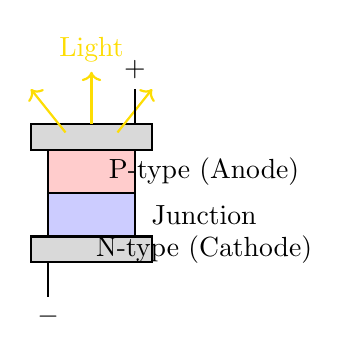
\begin{tikzpicture}[scale=1.1]
% LED structure
\draw[thick,fill=red!20] (1,2) -- (1,2.5) -- (2,2.5) -- (2,2) -- cycle;
\draw[thick,fill=blue!20] (1,1.5) -- (1,2) -- (2,2) -- (2,1.5) -- cycle;
\draw[thick,fill=gray!30] (0.8,2.5) rectangle (2.2,2.8);
\draw[thick,fill=gray!30] (0.8,1.2) rectangle (2.2,1.5);
% Labels
\node at (2.8,2.25) {P-type (Anode)};
\node at (2.8,1.75) {Junction};
\node at (2.8,1.35) {N-type (Cathode)};
% Light arrows
\draw[->,yellow!80!orange,thick] (1.5,2.8) -- (1.5,3.4) node[above] {Light};
\draw[->,yellow!80!orange,thick] (1.2,2.7) -- (0.8,3.2);
\draw[->,yellow!80!orange,thick] (1.8,2.7) -- (2.2,3.2);
% Terminals
\draw[thick] (1,1.2) -- (1,0.8) node[below] {$-$};
\draw[thick] (2,2.8) -- (2,3.2) node[above] {$+$};
\end{tikzpicture}
\end{center}

\textbf{Materials Used:}
\begin{center}
\begin{tabular}{|l|c|c|}
\hline
\textbf{Color} & \textbf{Material} & \textbf{Wavelength} \\
\hline
Red & GaAs & 700 nm \\
\hline
Green & GaP & 550 nm \\
\hline
Blue & GaN & 470 nm \\
\hline
\end{tabular}
\end{center}
\end{solutionbox}

\begin{solutionbox}
\textbf{Working:}
\begin{enumerate}
\item \textbf{Forward bias}: Electrons and holes recombine at junction
\item \textbf{Energy release}: Photons emitted during recombination
\item \textbf{Light color}: Depends on band gap energy
\item \textbf{Efficiency}: High electrical to optical conversion
\end{enumerate}

\textbf{Applications}: Displays, indicators, lighting, optical communication
\end{solutionbox}

\begin{mnemonicbox}
``LED: Light Emitting Diode, Electrons and holes Dance to make Light''
\end{mnemonicbox}

\vspace{15pt}
\begin{center}
\rule{0.8\textwidth}{0.4pt}\\[5pt]
{\large\textbf{--- End of Solutions ---}}\\[3pt]
{\small Modern Physics (DI01000061) -- Winter 2024}
\end{center}

\end{document}
